\epigraph{바트! 대학원생 놀리지 말거라.\\그냥 잘못된 선택을 한 것 뿐이야.}
{\textit{$\langle$The Simpsons$\rangle$,\\ \textsc{Marge Simpson}}}
% Tikz Reference: http://www.texample.net/tikz/examples/transparent-png-overlay/
\begin{tikzpicture}[remember picture, overlay]
    \node[inner sep=0pt] at (1.in,0.9in) {%
        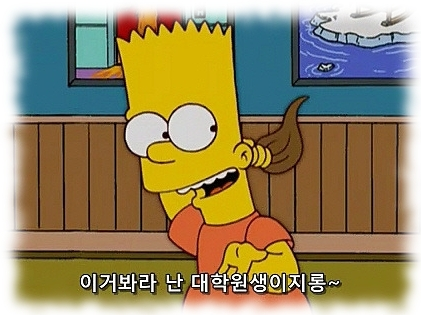
\includegraphics[width=2.4in]{./Figures/bart.jpg}%
    };%
\end{tikzpicture}
\begin{tikzpicture}[remember picture, overlay, opacity=0.8]
    \node[inner sep=0pt] at (2.7in,1.08in) {%
        
\includegraphics[width=1.2in]{./Figures/marge.jpg}};%
%    \draw[red,ultra thick,rounded corners] (2.in,1.28in) rectangle (1.2in,2in);
\end{tikzpicture}

\section{지도 교수 선정 및 팀 소개}
모 선배님 왈.. 지도 교수님을 선정하는 것은 배우자를 선택하는 것만큼이나
중요하다!! 매일 얼굴을 보고 학위 과정 중 매우 중요한 연구에 대해 이야기를 나누며
졸업 후에도 연구 내외적으로 관계가 평생 유지되기 때문이다. 이와 같이 매우 중요한
지도교수님을 선정하게 되는 과정에 대해 얘기를 해보자.

기존의 지도 교수 선정은 입학하자마자 ‘난 이 교수님을 택하겠어!’라는 다짐(?)과
함께 행정실 조교님께 메일을 보내고, 교수 회의를 통해 결정되면 끝나는 매우 단순한
과정이었다. 하지만 대학원 신입생들이 어떤 교수님이 어떤 연구를 하시는지 자세히 알
수 없어 이 과정이 부적절하다는 결론이 내려졌다. 그래서 2012년 2학기
신입생들부터는 지도 교수 선정 과정이 한 학기 뒤로 미루어졌다. 신입생들은 입학
직후에 해당학기 학과장 교수님을 지도 교수님으로 하여, 첫 학기에는 개별 지도
교수님 없이 수업을 듣게 된다. 대학원 생활 첫 학기에는 신입생 세미나인 ‘현대
천문학 특강’이라는 과목을 듣게 되는데, 이 과목에서는 매주 다른 교수님들이
들어오셔서 각 교수님의 현재 연구 주제 등에 대해서 알려주신다. 이러한 신입생
세미나 과목을 들으면서 자신의 관심 분야와 일치하는 교수님이 어떤 분인지를 생각해
보고, 학기가 끝날 때 쯤 행정실 조교님이 보내주시는 지도 교수 선정 관련 메일에
답장을 드리면 된다. 물론 이 수업을 통해 교수님들의 연구에 대해 많은 것을 알 수
있지만 연구실 분위기나 교수님의 스타일 등에 대해서 알기는 쉽지 않으므로 각
연구팀의 선배들에게 질문을 하고 조언을 구하는 것도 아주 좋은, 혹은 굉장히 필요한
방법이라고 할 수 있겠다. \\

자, 그렇다면, 서울대학교 천문학과의 각 연구팀에 대해 알아보자.

\subsubsection{구본철 교수님 팀}
\begin{figure}
\begin{center}
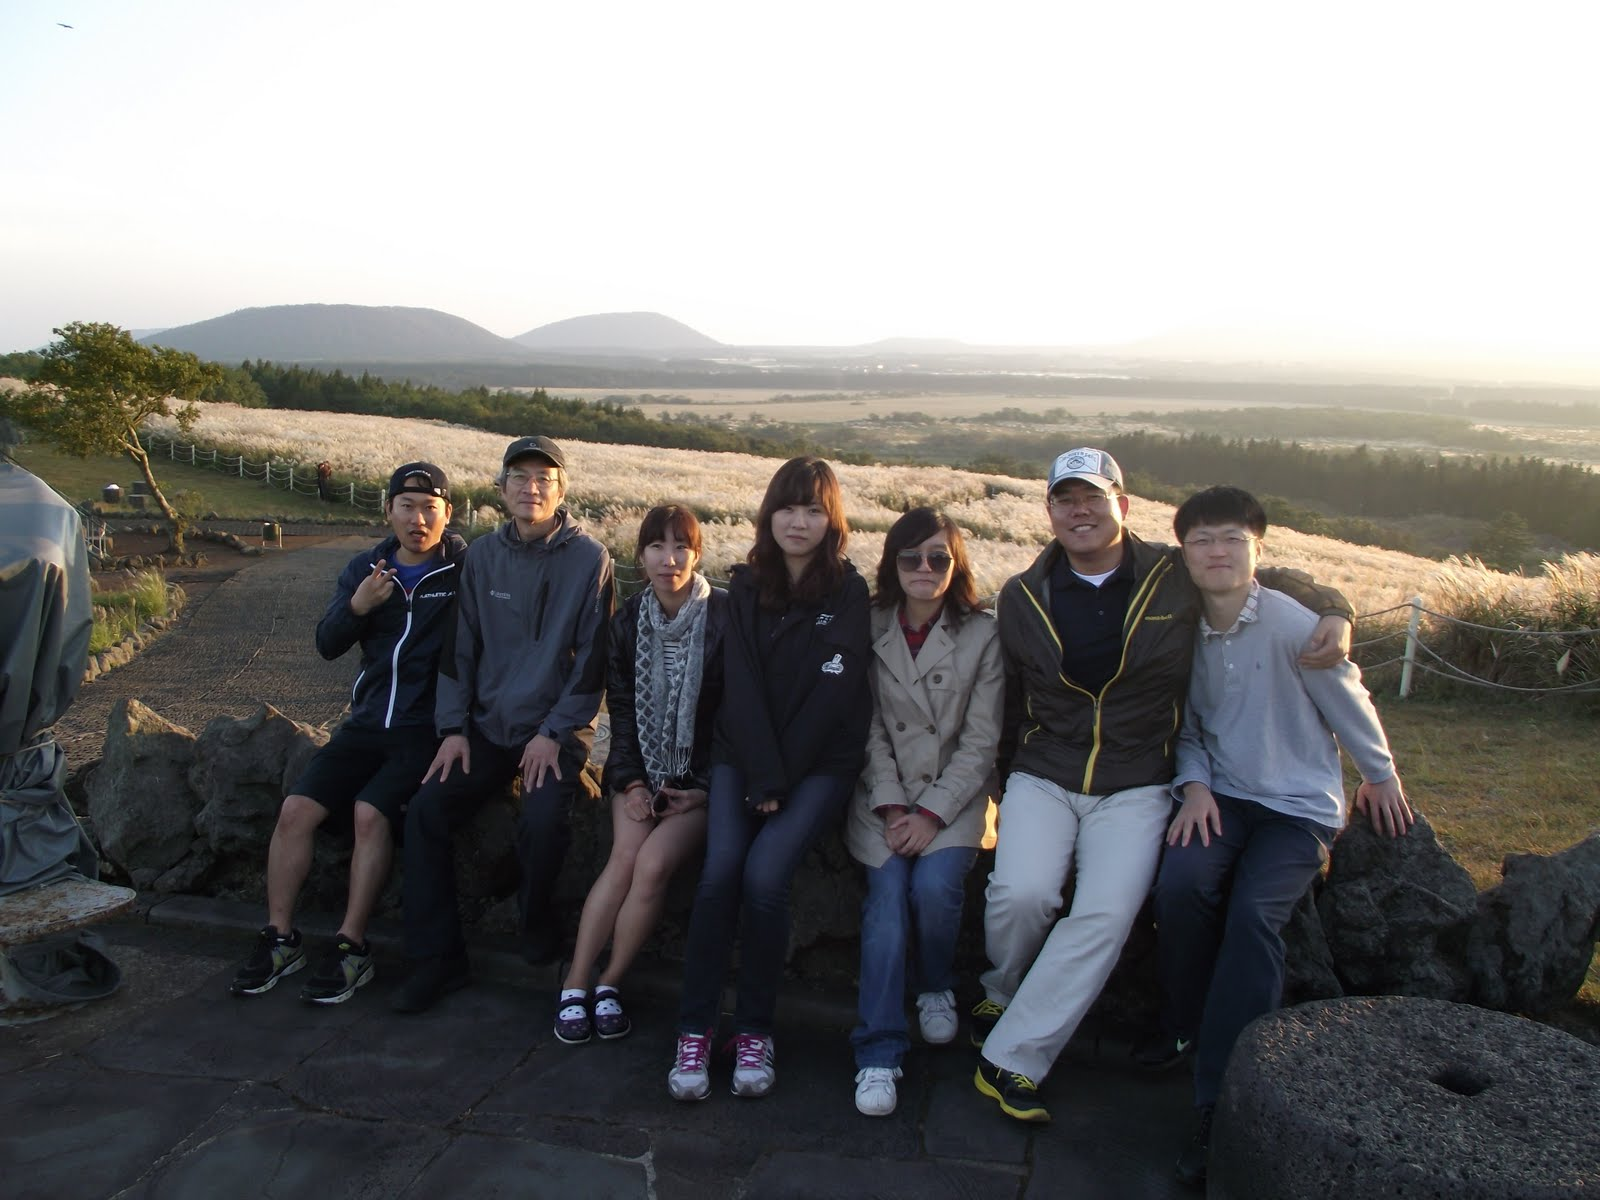
\includegraphics[width=0.85\textwidth]{./Figures/team-koo.jpg}
\legend{\textsf{구본철 교수님 팀---2011년 가을 제주도에서}}
\end{center}
\end{figure}
구본철 교수님 예하 팀 구성원들은 다양한 관측 자료를 이용하여 작게는 별의 탄생과 죽음에서부터 크게는 우리은하 내 성간물질의 구조와 진화에 이르는 광범위한 분야에 대해 관심을 가지고 다음과 같이 폭넓은 연구를 진행해 오고 있습니다.
\begin{packed_enum}
\item 우주망원경인 AKARI, Herschel, Spitzer 와 지상망원경인 AAT, Palomar, UKIRT 등으로부터 확보한 적외선 이미징 및 분광 자료를 활용한 별 탄생지역과 초신성잔해 연구. 
\item I-GALFA 서베이 자료와 SRAO 의 전파 관측 자료를 이용한 우리은하 중성수소의 구조 및 초신성잔해와 CO 분자운과의 상호작용에 대한 연구. 
\item 초신성 잔해의 진화, 성간난류 및 별 생성 등에 대해 수치 계산을 통한 이론연구
\end{packed_enum}
이러한 연구들은 한국천문연구원(KASI), 일본 우주항공연구개발기구(JAXA), 아레시보 전파관측소, 토론토 대학교 등 국내외 대학 및 연구소들과의 활발한 연구교류로 이루어지고 있어 수준 높은 연구 성과를 이루어내고 있습니다. 그리고 최근에는 한국천문학자들의 주도로 진행되고 있는 GEMS0 (Galaxy Ecology and Massive Stars at z=0) 및 IGRINS (Immersion Grating Infrared Spectrograph) 연구 그룹에 구본철 교수님과 팀 구성원들이 직, 간접적으로 참여하고 있어 앞에서 소개한 연구주제에 대해 보다 심도 있는 (근)적외선 연구가 이루어질 것으로 기대하고 있습니다.

2014년 3월 기준으로 팀 구성원은 구본철 교수님을 비롯해 박사 과정생 6명으로 이루어져 있습니다. 우리 팀은 연구 및 학업 상담을 위해 주 1회 정도로 교수님과 개별면담을 가지고 있고, 팀원들과의 연구교류 및 토의를 위해 월 1회 정도 팀 미팅을 가지고 있습니다.

\subsubsection{이형목 교수님 팀}
이형목 교수님 팀은 Infrared Astronomy, N-body particle simulation, Gravitational-Wave 등 매우 다양한 주제들을 연구하고 있습니다.

\begin{packed_item}
\item \textbf{Infrared Astronomy}
\begin{packed_item}
\item AKARI Space Telescope: 이형목 교수님은 한국 적외선 천문학 연구의 수장을 수년간 맡아 오셨고 지난 10년 가까이 일본의 AKARI 우주적외선망원경 일에 한국측의 리더를 맡고 계십니다. 그 중 Large Area survey 중 하나인 황도북극(NEP)관측 데이터 처리/분석을 하고 계시며 NEP 데이터는 Deep과 Wide 두 가지로 구분되는데, Deep은 일본, Wide는 한국이 맡아서 일하고 있습니다.
\item CIB (Cosmic Infrared Background): 최초의 별은 아주 멀리 떨어져 있음에도 불구하고 오늘날의 별에 비해 더 무겁고 밝기 때문에, 적색편이 된 그들의 영향이 오늘날 적외선 영역에 그 흔적을 남길 것이라는 몇몇 이론 연구와 간접적인 관측결과들이 있습니다. 그런 흔적은, 적외선으로 본 하늘의 밝기나, 밝기의 요동으로 나타날 것 입니다. 따라서, 적외선 배경을 연구하는 것은 우주 초기 천체의 형성과, 진화를 연구하는데 중요하다고 할 수 있습니다.
\end{packed_item}

\item \textbf{N-body Simulation}: 컴퓨터 시뮬레이션을 이용하여 많은 별들로 이루어진 다양한 천체의 역학적 진화를 연구합니다. 그 대상은 태양계부터 성단, 은하, 은하단 그리고 거대 구조까지 다양합니다. 최근에는 중력파의 중요한 대상인 compact binary formation에 대한 연구를 하고 있습니다.

\item \textbf{Gravitational-Wave}: 이형목 교수님은 앞으로 다가올 중력파 천문학시대를 개관 할 한국의 유일무이한 그룹인 한국중력파연구협력단 (Korea Gravitational-Wave Group, KGWG)의 단장님입니다. 아인슈타인의 일반상대론이 예견한 중력파의 존재에 대해 실제로 국제 중력파 연구기관(LSC:LIGO/VIRGO Scientific Collaboration)과 MOU를 체결하여 중력파 파형 Data분석, 후속광학관측 등의 연구를 하고있습니다.
\end{packed_item}
현재 박사과정 학생 4명이 있습니다. 일주일에 한 번씩 팀미팅을 통해 각자 연구한 것을 발표하고 토론하는 시간을 갖습니다.

\subsubsection{이명균 교수님 팀}
\begin{figure}
\begin{center}
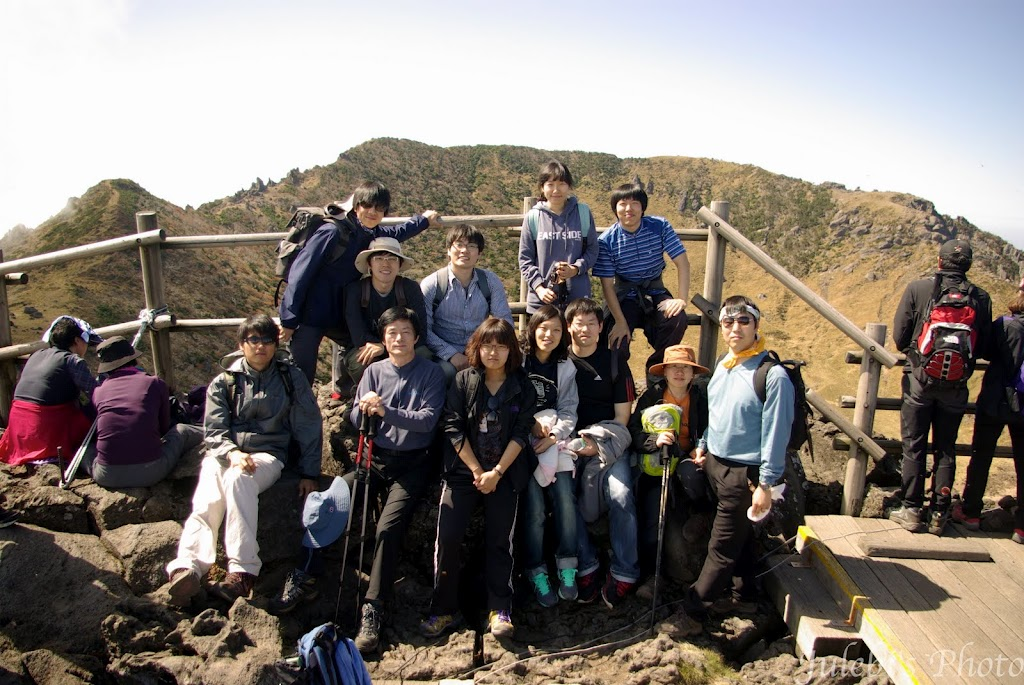
\includegraphics[width=0.85\textwidth]{./Figures/team-lee.jpg}
\legend{{\textsf{이명균 교수님팀---2011년 가을 한라산 등반}}}
\end{center}
\end{figure}
이명균 교수님 팀은 관측 우주론 (Observational Cosmology) 팀으로 천문학과 대학원에서 가장 규모가 큰 팀 중 하나입니다. 인자한 미소와 따뜻한 마음을 보여주시는 이명균 선생님의 지도 아래 2014년 1월 현재,  6명의 박사 과정생, 2명의 통합 과정생이 마치 형제들(!, 유경아 미안…)처럼 똘똘 뭉쳐 연구하고 있습니다.

관측 우주론 팀의 연구 분야는 1) 가까운 우주의 은하들 안의 AGB 별 2) 우리 은하의 산개 성단 및 구상 성단 3) 외부 은하의 성단계, 4) 외부 은하의 HII region, 5) 막대 은하의 형성과 진화 6) 은하 진화와 은하 환경의 관계 7) 다양한 환경에서 활동성 은하핵 특성 등으로 관측 우주론을 광범위하게 아우르고 있습니다. 이러한 주제에 대하여 주로 다양한 파장에서 얻은 측광 자료 분석과 보조적으로 분광 자료 분석을 통해 연구를 수행하고 있습니다.

관측 우주론 팀은 천문학과 대학원에서 팀 활동이 가장 활발한 팀입니다. 일단 매주 4시간 (ㅎㄷㄷ)에 이르는 팀 미팅을 통해 서로의 연구에 대한 열정적인 토론이 이루어집니다. 교수님과 학생들은 수시로 면담을 통해 연구 진행 상황을 논의하고, 졸업한 선배들과도 skype 등을 이용해 지속적인 토의 시간을 같습니다. 또한 1년에 한 두 차례 팀 워크샵을 개최하여 열띤 토론과 함께 아름다운 강산 (ex. 지리산, 울릉도, 제주도) 곳곳을 누비며 호연지기를 기르기도 합니다. 특히 등산에 있어서는 교수님의 지도 아래 모두가 달인이 되어가고 있습니다. 전국 명산들의 최고봉을 오르며 심신을 다스리며 팀워크를 다지고, 연구 의욕을 불사릅니다. 또한 정기적인 회식으로 팀 구성원들 사이의 돈독한 정을 자랑하기도 합니다. 조금 더 자세한 정보는 관측 우주론 팀 홈페이지(\url{astro.snu.ac.kr/~obscos}), 이명균 교수님의 홈페이지(\url{astro.snu.ac.kr/~mglee})를 통해 확인할 수 있습니다.

\subsubsection{박용선 교수님 팀}
박용선 교수님 팀은 성간 분자선을 관측하고 수치계산을 해서 은하 내 천문현상을 연구하고 있습니다. 또한  230GHz 전파망원경 (SRAO)을 운영하고 있으며, 천문기기개발을 하고 있습니다. 현 구성원은 교수님과 5명의 박사과정 학생, 2명의 석사과정 학생입니다.

우리 팀은 CO, CS를 비롯한 여러 분자선들을 SRAO, KVN등의 전파망원경을 이용하여 관측하여 분자운의 특성, 메이져선 관측을 통한 만기형 별의 특성, 복사 전달 방정식을 이용한 광 해리지역의 시뮬레이션을 주제로 연구하고 있으며, 미세전자기계거울(MEMS)을 이용한 적응 제어 광학계(Adaptive Optics)개발, 여러 배열 안테나의 빔을 적절하게 형성하여 태양풍을 측정하는 시스템 개발을 수행하고 있습니다. 우리 팀의 연구원들은 대부분 48-1동 전파천문대에서 생활하고 있고, 한 달에 한 차례 전파천문대에서 팀 미팅을 갖습니다.

\subsubsection{채종철 교수님 팀}
% \begin{figure}
% \centering
% \hspace*{\fill}
% \includegraphics[width=0.48\textwidth]{./Figures/2.jpg} \hfill \includegraphics[width=0.48\textwidth]{./Figures/3.jpg}
% \hspace*{\fill}
% \legend{(왼쪽) {\textsf{교수님 생신날 졸업한 선배들과}} (오른쪽) {\textsf{2012년 겨울}} } \label{fig:mult1}
% \end{figure}
\begin{figure}
\centering
\begin{minipage}{0.50\textwidth}
  \centering
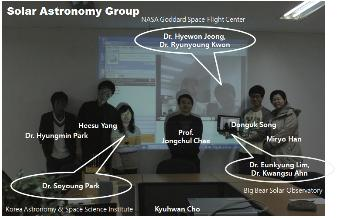
\includegraphics[width=\textwidth]{./Figures/team-chae-1.jpg}
\legend{{\textsf{채종철 교수님 생신 선배들과 함께}}} \label{fig:mult2}
\end{minipage}
\hfill
\begin{minipage}{0.48\textwidth}
  \centering
 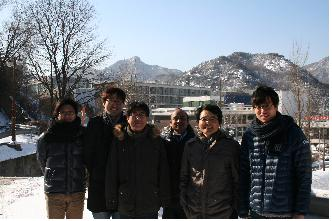
\includegraphics[width=\textwidth]{./Figures/team-chae-2.jpg}
\legend{{\textsf{채종철 교수님 팀---2012년 겨울}}} \label{fig:mult3}
\end{minipage}
\end{figure}

채종철 교수님 팀은 천문학과에서 유일하게 낮에만 관측을 할 수 있는 태양천문학 그룹(SNU Solar Astronomy Group)으로 현재 미국 빅베어 태양천문대 및 한국 천문연구원과 함께 태양의 광구, 채층, 그리고 코로나에서 일어나는 다양한 현상들을 분석 연구하고 있습니다. 현재 우리 팀의 구성원은 지도 교수님이신 채종철 교수님과 박사 후 연구원 2명을 비롯하여 박사과정 1명, 석·박 통합과정 2명과 석사과정 1명이 소속되어 있습니다.

또한 우리 팀은 태양의 관측 연구 이외에도 천문학 연구에 있어 매우 중요한 관측 기기에 대해서도 관심을 가지고 직접 개발하고 있으며, 2010년에는 고속 이미지 태양 분광기(FISS: Fast Imaging Solar Spectrograph)를 우리 팀에서 자체 개발하여 미국 빅베어 태양천문대(1.6m 태양망원경)에 설치를 하였습니다. 2010년 이후, 매년 6, 7, 8, 9월 약 4달 동안 우리 팀원들이 직접 가서 FISS를 사용한 관측이 이루어지고 있으며, 이 자료들을 사용하여 현재 좋은 결과를 얻고 있습니다. 

우리 팀은 매주 한 번의 팀 미팅을 통해서 서로의 연구 결과에 대한 다양한 토론을 하고 있으며, 매주 한번 있는 논문 쓰기 연습 시간을 통해서 논문 작성법에 대한 공부를 하고 있습니다. 또한 2주에 한번 있는 한국 천문연구원과의 미팅을 통해서 서로의 연구 활동을 공유하며, 미국 빅베어 태양천문대 및 한국 천문연구원과의 워크샵을 통해서 연구 활동 및 결과 그리고 관측 기기 개선을 위한 정보를 공유합니다.

채종철 교수님 연구실은 19동 310호에 위치하고 있으며, 연구 분야에 대한 자세한 정보는 다음을 참고해 주세요. 교수님 홈페이지 : \url{http://astro.snu.ac.kr/~chae} , FISS 홈페이지 : \url{http://fiss.snu.ac.kr}

\subsubsection{임명신 교수님 팀}
\begin{figure}
\begin{center}
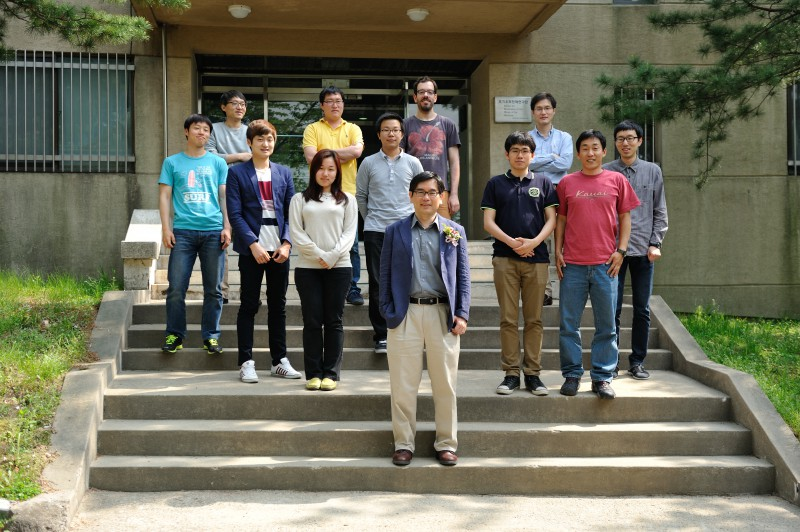
\includegraphics[width=0.85\textwidth]{./Figures/team-im-2014-1.jpg}
\legend{{\textsf{임명신 교수님 팀---2013년 스승의 날}}}
\end{center}
\end{figure}
임명신 교수님은 초기 우주 천체 연구단(Center for the Exploration of the Origin of the Universe, CEOU)의 단장님 입니다. 초기 우주 천체 연구단은 서울대의 김웅태 교수님, 경희대의 박수종 교수님 연구팀과 함께, 초기 우주에 존재하였던 (빅뱅 이후 ~1Gyr 지났을 때) 천체들을 발견하고 그것들의 성질을 연구하는 Infrared Medium-deep Survey (IMS)를 진행하고 있습니다. 
우리 팀에는 현재 교수님 이외에 박사후연구원 3분을 비롯하여 대학원생 8명, 행정간사 1명이 소속되어 있습니다.

우리 팀의 연구 대상은 가까운 우주에서부터 멀리 있는 우주, 즉 초기 우주에 존재하는 보통 은하, 활동성 은하, 초거대질량 블랙홀, 감마선 폭발 천체 등입니다.
\begin{packed_enum}
\item 보통 은하(Normal Galaxies): 무거운 타원은하(Elliptical Galaxies)의 색구배(Color Gradient)와 질량 대 광도 관계(Fundamental Plane), 매우 붉은 은하(Extremely Red Objects)의 군집. 초기 은하단의 발견(Overdensities of Proto-Clusters), 초은하단(Super Cluster)의 성질 연구. 초기 우주 별생성은하(Star-forming Galaxies)의 별 탄생률(Star Formation Rate) 연구, 표면밝기가 어두운 은하(Low Surface Brightness Galaxy) 연구.
\item 활동성 은하(Active Galaxies) 및 초거대질량블랙홀(Super Massive Black Holes): 초기 우주의 퀘이사(Quasars) 발견, 초거대블랙홀의 질량 진화, 초기 우주의 은하간 물질(Intergalactic Medium) 이온화 연구. 적외선 방출선을 이용한 블랙홀 질량 측정법, 붉은 활동성 은하핵(Red AGN) 발견 및 연구, 전파 활동성 은하핵 연구(Radio AGN Properties). 활동성 은하의 별 생성률 지표(Star Formation Rate Indicator). 은하 합병이 블랙홀 질량에 미치는 영향 연구.
\item 감마선 폭발 천체(Gamma Ray Bursts): 감마선 폭발 천체의 가시광 및 적외선 후속 관측(Follow-up). 블랙홀 활동 모니터링(Long Term Monitoring of BH Ignition). 감마선 폭발 천체가 속해있는 은하의 먼지의 기원(Dust property of GRB Host Galaxy).
\item 외부 은하에서 발견되는 초신성: 초신성 후속 광도 변화 관측(SN Follow-up Observation). M101은하에서 터진 초신성 모니터링(M101SN Observations).
\end{packed_enum}
이러한 천체들을 지상의 다양한 망원경(주로 UKIRT, McDonald 2.1m, Maidanak 1.5m, LOAO 1.0m 등) 혹은 우주 망원경(AKARI 등)을 이용하여 관측을 합니다. 우리의 연구에 필요한 기기를 직접 개발하기도 하는데, 예를 들어, 우리가 만든 SNUCAM이 Maidanak 1.5m 망원경에, CQUEAN이 McDonald 2.1m 망원경에 부착이 되어 있습니다. 또한 우리 팀은 매일 아침 arXiv 에 올라오는 논문들을 리뷰합니다. 흥미로운 논문들을 같이 읽고 내용에 대해 의논 합니다.

우리 팀의 연구실은 다른 팀들과는 다르게 19동이 아닌 45동에 위치하고 있습니다. 연구 분야에 대한 자세한 정보는 다음을 참고해 주세요. (팀 홈페이지: \url{http://astro.snu.ac.kr/~exact} , CEOU 홈페이지: \url{http://bigbang.snu.ac.kr} , 교수님 홈페이지: \url{http://astro.snu.ac.kr/~mim})

\subsubsection{김웅태 교수님 팀}
김웅태 교수님 팀은 천문학과에서 좀처럼 찾기 힘들다는(?) 이론, 수치계산 그룹(CNTAG: Computational aNd Theoretical Astrophysics Group)으로 초기우주천체연구단(CEOU)에 속해 있습니다. 현 구성원은 교수님과 3명의 박사과정 학생, 1명의 석사과정 학생입니다.
  김웅태 교수님을 비롯한 그룹원들은 이론과 수치계산의 방법을 이용해 천문학의 다양한 문제를 연구합니다. 최근의 연구 주제는 막대 은하, 막대-나선 은하에서의 기체역학과 별 형성, 기체 원반의 중력 불안정, 우리 은하의 나선팔 구조 등이며, 특히 은하 기체 역학, 별 형성의 연구는 미국 프린스턴대학 대학의 이론, 수치계산 그룹들과 공동연구를 진행하고 있습니다. 그 밖에도 나선팔에서의 거대분자구름 형성, 동역학적 마찰, 격변 변광성에서의 질량 교환, 은하단 기체역학 등의 여러 문제에 관심을 갖고 있습니다.
  그룹원들은 한 달에 한 번씩 갖는 팀미팅을 통해 서로의 연구 활동과 관심사를 공유하며, 매년 하반기에는 KNAG(Korean Numerical Astrophysics Group) 정기 미팅에 참가하기도 합니다.

더 자세한 정보는 교수님 홈페이지 (\url{http://astro.snu.ac.kr/~wkim}), CNTAG 홈페이지 (\url{http://astro.snu.ac.kr/cntag})에서 찾아볼 수 있습니다.

\subsubsection{이정훈 교수님 팀}
 이정훈 교수님 팀은 한국의 여러 대학의 천문학과에서 찾아보기 힘들다는 이론 우주론 팀입니다. 현재는 교수님과 1명의 석박사 통합과정 학생으로 구성되어 있습니다. 이론 우주론 팀에서는 주로 우주의 거대구조의 특성과 진화를 이론적으로 연구하여 우주표준모형($\mathrm{\Lambda CDM}$: Lambda-Cold Dark Matter Model)의 유효성을 검증하는  연구를 합니다. 은하나 은하보다 더 큰 거대구조 (은하단, 필라멘트, 보이드)의 질량함수 및 분포의 이론적 모델을 세우고 관측적, 수치적 자료를 함께 이용하여 암흑물질과 암흑 에너지, 우주 초기 밀도장의 성질을 규명합니다. 
 또한 우주 표준모형으로 설명되지 않는 여러 관측적인/ 수치적 현상을 설명하기 위해 기존의 모형의 보완 및 새로운 모형의 제안과 검증 과정이 이론 우주론 팀의 주요 연구 주제 중 하나입니다. 미국, 독일, 캐나다 등지의 저명한 우주론 학자들과 활발한 공동 연구를 펼치고 있습니다. 학생들의 연구는 주로 교수님과의 개별 면담을 통해 진행되고 한 학기에 한두번 정도의 비정기적인 팀 미팅을 갖습니다. 필요에 따라 우주론 팀의 학생들끼리 모임을 갖기도 하였는데, 이 또한 비정기적인 모임으로 자세한 정보는 이론 우주론 팀에 소속된 학생에게 문의해주시기 바랍니다.

\subsubsection{우종학 교수님 팀}
우종학 교수님 팀은 우주에서 가장 강력한 에너지원인 거대질량블랙홀들과 은하의 형성 및 진화에 대해 연구하는 거대블랙홀 연구실(AGN Research Group) 입니다. 현 구성원은  우종학 교수님과 박사 후 연구원 한 분과 박사과정 2명, 석사과정 1명입니다.

거대질량블랙홀은 은하 중심에 위치하는 것으로 알려진 질량이 태양질량의 백만배 가량을 넘어가는 천체입니다. 이러한 블랙홀로 가스가 유입될 때 일어나는 현상인 활동성은하핵(AGN:Active Galactic Nucleus)은 수천억 개의 별들로 이루어진 은하 전체의 밝기보다 열배에서 백배 가량 더 많은 에너지를 방출합니다. 거대블랙홀 연구실에서는 블랙홀과 AGN, 그리고 은하의 진화과정을 밝히기 위해 허블우주 망원경, Keck 망원경, Palomar 망원경, Lick 망원경, Subaru 망원경, SALT 망원경 (The Southern African Large Telescope) 등을 비롯한 다양한 관측기기를 이용하여 퀘이사, 세이퍼트(Seyfert) 은하, 전파 은하 등을 연구하고 있습니다.

저희 팀은 보통 매주 팀미팅을 가지고 있습니다. 팀미팅 시간은 주로 한 사람이 연구와 관련된 논문을 리뷰하고 이에 대해 각 팀원들과 교수님이 토의하는 방식으로 이루어집니다. 또한 간단히 연구결과를 이야기하는 시간도 있어 서로의 연구가 어떻게 진행되어가고 있는지를 알 수 있습니다. 
(우종학 교수님 홈페이지 : \url{http://astro.snu.ac.kr/~woo})

\subsubsection{이시구로 마사테루 (Ishiguro Masateru) 교수님 팀}
이시구로 선생님 팀은 태양계 천문학을 연구하는 팀입니다. 저희 팀은 한국에서 태양계를 공부하고 싶으신 학생들의 몇 없는 선택지 중 하나이고, 행성과 달을 제외한 태양계 천체를 공부하고 싶으신 분들께는 슬프게도(?) 유일한 선택지입니다. 2014년 봄학기에는 선생님 외에 기존의 학생 중 1명의 박사과정 학생과 1명의 석사과정 학생, 1명의 통합과정 학생이 남아있을 것입니다.

태양계 천문학 연구에서는 여타의 천문학 분야보다 훨씬 자세한 관측 자료를 얻을 수 있으며, 제한되나마 실제 샘플도 획득할 수 있습니다. 그 결과, 여타의 분야보다 상대적으로 복잡하고 구체적인 모형이 제시, 검증되고 있습니다. 저희 팀에서는 이러한 상황에 대응하기 위하여 다양한 연구 방법을 이용하고 있습니다. 관측, 수치 실험, 기기 제작 등의 연구 방법을 종합적으로 동원하여, 넓은 안목에서 태양계의 구체적 존재 양태를 추적하고 있습니다. 실제로 8m 급 대형망원경, 다양한 2m 급 중형 망원경, 저희 팀에서 직접 제작 중인 소형 광학기기를 이용하여 딥필드에서 전천까지, 자외선에서 적외선까지, 측광, 분광, 편광 관측을 수행하고 있으며, 이와 병행하여 수치 실험도 동시에 진행되고 있습니다. 지금 입학하시는 분이 박사학위를 준비하시게 될 수년 후에는 선생님이 개발에 깊이 참여하고 있는 소행성 탐사선 Hayabusa II가 획득한 자료도 우선적으로 이용할 수 있을 것입니다.

현재 저희 팀에서 수행하고 있는 구체적 연구 주제를 예로 들면 다음과 같습니다.
\begin{enumerate}
\item 지구 근처에 존재하는 천체들의 기원과 특징은 무엇인가?
\item 혜성과 소행성이 충돌을 겪으면 어떠한 일이 발생하는가?
\item 태양계에 존재하는 티끌의 구체적 기원은 무엇인가?
\item 혜성과 소행성에서 발생한 티끌들이 그 후 어떻게 진화하는가?
\end{enumerate}
위와 같은 연구를 종합하여 태양계의 기원과 진화를 종합적으로 이해하는 것이 저희 팀의 목적입니다. 물론 구체적인 세부 주제는 계속하여 추가, 변경되고 있습니다.

저희는 보통 한 주에 한 번씩 3$\sim$4시간의 팀 미팅을 갖고 있으나, 얼마든지 변경의 여지가 있습니다.

\subsubsection{사샤 트리페 (Sasha Trippe) 교수님 팀}
사샤 트리페 교수님은 우리 과 외국인 교수님 투 톱 중 한 분으로 독일에서 박사학위를
받으신 후, 프랑스 IRAM에서 박사후과정을 거쳐 2011년에 서울대에
부임하셨습니다. 현재 네 명의 석박통합과정생을 두고 계시고, 연구는 주로 활동성
은하핵(AGN)을 전파영역으로 분석하여 수행하고 있습니다. 연구수행에는 주로 21m
망원경 세 개로이루어진 한국 VLBI망(KVN)과, 한국(KVN)-일본(VERA: 20m 망원경 7개)
연합 VLBI망(KaVA)을 이용하고 있습니다. 또한 교수님은 Modified Newtonian
Dynamics에도 관심이 있으시고, 기기 개발 방면에도 흥미를 갖고 계십니다. 교수님
홈페이지를(\url{astro.snu.ac.kr/~trippe}) 방문하시면 찾아보시면 재미있는 내용들을
찾아보실 수 있습니다.


\subsubsection{윤성철 교수님 팀}
윤성철 교수님 팀은 국내에 몇 없는 Stellar Astrophysics, 즉 항성의 내부 구조 및 진화, 탄생과 죽음을 연구하는 팀입니다. 윤성철 교수님은 2013년에 부임하셨고, 2014년 초 현재 석박통합과정생 두 명이 소속되어 있습니다. 교수님이 매우 젊으시고 부임 초기이시기 때문에 굉장히 열려있으시고 열정적이시며, 항성진화 뿐만 아니라 다양한, 말그대로 `다양한’ 분야에 폭넓은 관심을 갖고 계십니다.

현재는 우주 초기의 별(Pop III)의 탄생이나 He별의 진화와 같은 다양한 항성들의 진화뿐만 아니라, Type Ib/ Ic 초신성 폭발이 발생할 수 있는 조건과 같은 항성 전반과 관련된 총체적 특성들을 항성진화 모델통해 컴퓨터 계산으로 연구하고 있습니다. 

저희는 보통 매주 금요일에 팀미팅을 갖고 있으며, 이 외의 정보에 대해서는 교수님 홈페이지(\url{http://astro.snu.ac.kr/~yoon/home/})에서 찾아보실 수 있습니다.

\vspace{0.05\textheight}

\section{강의 소개 및 수업 관리}
대학원 합격의 기쁨을 누리기도 잠시, 신입생 여러분에게는 정식으로 입학하기 전에 미리 결정하고 해야 할 일들이 기다리고 있다. 그 중 빠뜨릴 수 없는 것은 바로 학기가 시작되면 어떤 수업을 들어야 하는지 알아보는 것이다. 새롭게 시작되는 대학원 생활을 앞두고 의욕에 가득 차 있을 당신! 하지만 첫 학기부터 단추를 잘 못 꿰게 된다면 억울한 일이 아닐 수 없다. 강의 정보 확인은 서울대학교 정보 광장 (\url{http://my.snu.ac.kr})에서 수강 편람에 들어가 강의 계획서를 열람하는 것이 가장 확실한 방법이지만, 한 학기에 개설되는 수업의 종류가 다양하기 때문에 사전 정보가 없이 선택하기란 쉬운 일은 아니다. 따라서 이 챕터에서는 신입생의 수업 선택에 도움을 주고자 간단한 강의 소개와 이수 규정에 대해 설명하도록 한다.

석박통합 과정의 졸업 이수 기준 학점은 총 60학점이다. 대학원에서는 수업과 더불어 연구도 진행해야 하기 때문에 통합과정의 수료를 6학기로 보고 있다면 한 학기에 10학점을 들어야 하기 때문에 빠듯할 수 있다. 이를 돕기 위해 18학점의 논문연구교과목과 6학점의 콜로퀴움 수업을 두어 24학점의 부담을 덜어주고 있으니 이를 참고하여 글을 읽자.

적합한 선택을 하기 위해서 가장 먼저 수업 종류에 대해 알아보자. 천문학과의 수업은 크게 일반 교과 수업과 세미나 수업으로 나누어 볼 수 있다.
\begin{packed_item}
\item 교과 수업은 학부 과정에서 수강했던 수업과 크게 다르지 않고 천문학 연구를 위한 배경지식을 습득하는 데에 주력하게 되며, 일반적으로 선생님의 강의로 수업이 구성된다. 수업 평가는 주로 시험을 통해 이루어지며 부가적으로 과제와 수업 참여도를 반영하기도 한다.
\item 반면 세미나 수업은 강의보다는 학생들의 발표와 토론이 주가 되는 과목이다. 자신의 연구 주제를 가지고 수업이 진행되는 동안 스스로 연구를 진행해야 하기 때문에 시험에 대한 단기적인 스트레스는 없는 편이지만 지속적인 발표와 레포트로 연구 능력과 성실함을 요구한다.
\end{packed_item}
 따라서 정해진 규정은 없지만 일반적으로 1학년 때는 주로 교과 과목에 투자를 하고, 1년 정도 지난 후에 세미나 수업을 들을 것을 추천하고 있다. 특강 및 세미나 수업을 듣기 전에 관련 수업을 미리 들어두는 것이 좋다 (예: 천체분광학 및 실험 $\rightarrow$ 천체분광세미나 ). 단, 지도 교수님에 따라 세미나 수업을 권유하는 분도 계시기 때문에 수강 신청 전, 팀 선배에 조언을 구하는 것은 언제나 도움이 된다는 점을 잊지 말자.

이와는 별도로 천체물리세미나(콜로퀴움) 수업과 논문연구교과목이 있다. 천체물리세미나는 학기 중 매주 목요일과 추가로 있는 특별 콜로퀴움에 참석하는 것으로 수업을 대체하는데, 박사과정 중 2번 신청할 수 있으며 담당 선생님에 따라 레포트를 요구하기도 한다. 논문연구교과목은 총 18학점을 대체할 수 있는 수업으로 강의나 발표 없이 개인의 연구 역량을 증진시키고 연구 시간을 확보하는 데에 도움을 준다. 따라서 통합과정 중 교과 과목과 세미나 수업으로 이수해야 할 학점은 총 36학점으로 12과목이 되겠으며 이는 6학기 동안 매 학기 두 과목을 들어야 하는 수준이다.
교과 수업의 간략한 설명은 학과 홈페이지의 \href{http://astro1.snu.ac.kr/home/kor/info/subject_dahakwon.asp?globalmenu=3\&localmenu=5}{학사정보 탭}에 있으니 참조하자. 
이 중 첫 학기 추천 과목은 봄 입학 기준 천문관측법과 천체물리학, 가을 입학 기준 외부은하와 우주론, 성간 물질과 항성역학 및 중력이며, 위 수업들은 논문자격시험의 필수 과목이기도 하다. 
이 밖에도 연구팀을 소개하는 신입생 대상 수업 ‘현대 천문학 특강’ 이 있으며, 배경 지식이 부족하다고 생각될 경우 학부 수업이나 타과 수업을 수강할 수도 있다.

\section{컴퓨터 세팅, 계정 만들기}
\subsection{하드웨어 마련하기}
책상 위에 펜과 종이, 커피 한 잔만 있으면 논문이 써지는 순수 이론가가 아니라면, 대부분의 연구 활동은 컴퓨터에서 이루어진다. 그러니 무엇보다 개인컴퓨터를 마련하는 것이 우선이다. 개인컴퓨터는 팀에서 지원해주기도 하니 반드시 미리 선배들을 통해 알아보자!

연구용으로 컴퓨터를 장만할 때 고려해야 할 사항이 있다. 시뮬레이션을 돌리거나 하는 많은 연산이 필요한 작업이 예상된다면 CPU 성능과 RAM 용량이 중요할 것이다. 만약 많은 양의 데이터를 처리해야 한다면 하드의 용량이 중요할 것이고, 이미지를 주로 봐야 한다면 큰 모니터 혹은 듀얼 모니터가 있으면 좋을 것이다. 하지만 만약 팀이 소유하거나, 외부 기관이 소유한 서버에서 작업을 주로 하게 된다면 CPU의 성능이나 하드의 용량은 그다지 중요하지 않을 수도 있다. 이와 같은 사항은 같은 팀의 선배나 지도교수님과 상의해보는 것이 가장 좋을 것이다.

\subsubsection{IP 신청}
학교 어디에서든 무선인터넷은 콸콸콸 터지고 19동에서도 astro 무선인터넷을 사용할 수 있다 (비밀번호는 선배에게 물어보라). 그러나 데스크톱의 네트워크 연결을 위해 IP는 반드시 필요하다. 개인 IP는 정보 광장에 접속해 신청할 수 있다. 그리고 IP신청을 하면 지도교수님에게 메일을 보내어 담당학생이 맞는지 확인을 한 후 IP를 발급해준다. 그러니 지도교수님에게 미리 말씀을 드리는 것도 잊지 말자. (서울대학교 포털 (\url{http://my.snu.ac.kr}) 로그인 --- 스누인지원 --- IT 서비스 --- IP/Domain 신청/반납)

\subsubsection{포트 신청}
집에서도 연구하는 성실한 학생임을 지도 교수님께 어필할 기회가 있다. 
바로 자신의 데스크탑의 포트를 여는 것이다. IP 신청과 마찬가지로 포트 신청을 하면 지도 교수님의 확인 후에 포트를 열어준다.
이 경우 지도 교수님께서, 아 이 학생은 집에서도 연구하는 성실한 학생이구나 하며 흐뭇한 미소를 지으실지도 모른다.
일단 IP 신청을 마치고 받은 후에 IP와 비슷한 경로를 통해 들어가 자신의 IP에 원하는 포트를 열어달라고 요청하자. 
(\url{http://my.snu.ac.kr}) 로그인 --- 스누인지원 --- IT 서비스 --- IP/Domain 신청/반납)
보통 많이 사용하는 포트는 21번 (FTP), 22번 (SSH), 5900 (VNC) 정도이다. 이 정도 포트를 열어두면 집에 있는 컴퓨터로 학교 데스크탑에 원격 접속하여 신나는 연구 생활을 즐길 수 있다!!! 

\subsubsection{공용 네트워크 프린터 설정}
학과에서 공용으로 사용하는 프린터는 3층 행정실 옆에 위치하고 있다. 연결 방법은 운영체제마다 조금씩 차이가 있다. 잘 모르겠으면 인터넷을 찾아보거나, 행정실 조교님 혹은 주변 선배에게 물어보면 친절히 잘 알려줄 것이다. 아! 왠만하면 잊지 말고 양면 인쇄 설정엔 체크하여 자원을 아끼자. 
\begin{packed_item}
\item 흑백프린터 - HP LaserJet 4515x (IP: 147.46.20.148)
\item 컬러프린터 - HP Color LaserJet 4700 (IP: 147.46.135.143)
\end{packed_item}

\subsection{소프트웨어 마련하기}
하드웨어를 마련했다면 이제 소프트웨어를 설치해보자. 천문학과에서 기본적으로 사용하는 프로그램은 다음과 같다.
\begin{packed_item}
\item IDL : 파일 입출력, 데이터 분석을 위한 프로그래밍 언어로 가장 널리 쓰인다.
\item IRAF : 리눅스에서 천문학 관련 작업(Task)들을 쉽게 처리 할 수 있도록 Package화 해놓은 Tool
\item PYTHON : 천문학계에서 IDL과 쌍벽을 이루는 고급 프로그래밍 언어, PYTHON으로 IRAF Task 들을 구현해 놓은 PYRAF라는 것도 있다.
\item LaTeX : 주로 논문을 작성하게 될 때 쓰게 되는 문서 작성 도구
\end{packed_item}
각 팀별로 사용하는 프로그램들이 다르고, 개인의 취향이 있으니 미리 알아보고 준비하도록 하자. 프로그램에 대한 자세한 내용은 3장에서 다루고 있으니 3장을 자세히 살펴보도록 하자.

팀 내 서버에서 주로 작업을 하게 된다면 원격 접속 프로그램이 필요하다.
\begin{packed_item}
\item Xmanager : 아래에서 설명하고 있는 캠퍼스 라이센스 S/W 중 하나로서 SSH protocol로 서버에 접속할 수 있는 환경을 제공해준다. (Xftp, Xstart 등)
\item VNC :  Remote Terminal (주로 자신의 Desktop) 에서 서버의 자신의 작업 공간 (주로 서버의 자신 계정의 홈페이지) 으로 접속하여 작업할 수 있게 해주는 프로그램이다.  VNC의 강력한 점은 Terminal로 접속하는 방식과 달리 자신이 했던 작업을 그대로 다음번 접속 때 이어서 할 수 있다는 점이다. (\url{http://www.realvnc.com})
\end{packed_item}

\subsubsection{캠퍼스 라이센스 S/W 배포 시스템}
교내 IP로 접속한 경우 학교에서 지원하는 각종 소프트웨어를 다운받을 수 있다. 학교 사이트에 접속하면 더욱 쉽고 편리하게 다양한 소프트웨어(Window, MS Office, Adobe 프로그램들, 보안프로그램 etc)를 다운받을 수 있다. (서울대학교 포털 로그인(\url{http://my.snu.ac.kr}) --- QUICK MENU --- SW 다운로드)

\subsection[E-mail 계정 만들기]{E-mail 계정 만들기\footnote{이준협 선배님의 매뉴얼로부터 \cite{manual_ljh}}}
천문학과에 입학하여 가장 먼저 필요한 것 중 하나는 학과서버에 자신의 계정을 만드는 것이다. 학과 사무실에 자기 계정으로 쓸 아이디를 적어내면 그 아이디로 계정을 만들어준다. 그런데 자기 이름의 이니셜을 이용해서 만들라는 권장사항을 무시하고 원래 인터넷에서 즐겨 쓰던 아이디를 고집하는 사람이 꼭 매년 한두명씩 나온다. 천문학을 중간에 그만둘 계획을 가지고 있지 않다면 절대 그러지 말기 바란다. 여기에 만드는 계정은 그대로 자신의 공식적인 메일주소가 되며 논문을 쓰면 논문에 그 메일주소를 실어야 된다. 그리고 어떤 천문학자도 자신의 이름과 무관한 이상한 아이디로 공식메일을 사용하지는 않는다. 가령 자신이 인터넷상에서 \texttt{sexyking}라는 아이디를 사용하고 있었다고 해서 그대로 학과계정을 만들면 논문저자 이름 밑에다가 \texttt{sexyking@astro.snu.ac.kr} 이라고 써야 하는데, 그걸 읽는 사람들이 어떻게 생각할지 상상해 보라. 공식 계정답게 무난하고 품위 있는 아이디를 만들기 바란다. 예를 들어 이름이 홍길동이라면 \texttt{gdhong} 으로 하는 것이 가장 일반적이며, \texttt{ghong, gildong, honggd, hgd} 등등까지는 대체로 무난하다고 하겠다.

\section{학자금 마련하기}
\begin{itemize}
\item \textbf{장학금 신청 시기}: 매년 마다 조금씩 틀리지만 일반적으로 2학기는 5월 첫째 주, 다음 해 1학기는 11월 첫째 주에 장학금 신청 카드를 제출해야 한다. 신청하지 않으면 장학금을 받을 수 없다!
\item \textbf{장학금 종류}: 강의$\cdot$연구 장학금 (GSI), 수업료 및 입학료 면제 장학금, 근로 장학금, BK 장학금, 유학생 장학금, 대출학자금이자지원 장학금, 서울대학교 발전기금 장학금, 이공계 국가장학금, 글로벌 박사 펠로우쉽, 미래 기초과학 핵심리더 양성사업, 교외 장학금 (롯데, STX, KT\&G 등) 등 여러 가지 종류의 장학금이 있다. 장학금, 학자금 대출과 관련한 자세한 사항은 다음의 사이트들을 참고하자 (\url{http://scholarship.snu.ac.kr/}, \url{http://www.nrf.re.kr}).
\item 행정실 조교님께서 학생들이 받을 수 있는 학내, 외부 장학금과 관련한 메일을 항상 보내주시니 \textbf{\emph{메일함을 수시로 체크하자!}}
\end{itemize}

\subsubsection{올림피아드 조교}
학과 건물 내에 올림피아드 사무실이 위치하고 있기 때문에 종종 시험감독, 채점 조교를 모집할 때가 있다. 짧은 시간을 일하고도 짭짤한 수입을 얻을 수 있기 때문에 용돈 벌이에 좋을 것이다.


\section{주거 관련 정보}
\begin{packed_item}
\item 현재 대학원생들은 기숙사/서울대 입구/녹두/낙성대에 거취함. (물론 집이 가까운 사람은 집에 거주한다!)
\item 기숙사에 대한 자세한 정보는 사이트를 참고하자!! (\url{http://dorm.snu.ac.kr})
\item 기숙사 신청 기간을 놓치면 입사할 수 없으니  사이트를 수시로 체크하자!! 대부분 방학 전에 신청하므로 잊지말자!!
\item 천문학과 홈페이지에도 공고한다. 하지만 혹시 모르니 항상 사이트를 체크하자!!
\item 참고로 까다롭지 않지만 기숙사 입사조건이 있다. (성적, 건강검진, 보호자 거주지 등)
\item 아래의 그림은 기숙사 신청시 홈페이지이다. 아래의 그림에서 붉은색 BOX 안에 있는 내용을 체크하지 말자!! 대학원 신입생은 붉은색 BOX 안의 내용에 해당되지 않으므로 체크하면 기숙사 입사와 멀어진다. 경험자 있음..;;;
\item 기숙사에 떨어진 사람은 자취나 하숙을 하게 되는데 방 값은 일반적으로 서울대입구역=낙성대 $>$ 녹두(신림9동) 이다.
\item SNULIFE 사이트의 생활정보 카테고리에 스누복덕방에서 다양한 방을 알아 볼 수 있다. 링크: \url{http://www.snulife.com/housing}
\item 자취나 하숙보다는 기숙사를 추천하니 기숙사 입사를 위해 최선을 다하자!!
\item 더 자세한 정보는 서울대학교 생활 백서를 참고하자 (2009년 버전으로 현재와는 조금 다를 수 있다)!! 링크: \url{http://www.snuco.com/html/partner/partner_white_papaer.asp}
\end{packed_item}

\begin{figure}
\begin{center}
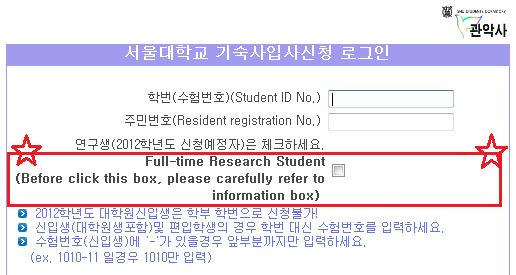
\includegraphics[width=0.85\textwidth]{./Figures/dorm.png}
\legend{{\textsf{붉은색 BOX 체크하지 말것!}}}
\end{center}
\end{figure}


